\documentclass[12pt,twoside]{article}

% La extensión total de la memoria deberá ser de un máximo de 50 páginas (excluidos resumen, índice y posibles anexos).

% Según las recomendaciones de estilo, el formato de la memoria se ajustará a lo siguiente:
% - Formato del papel: DIN A4.
% - Impresión a dos caras.
% - Márgenes: superior e inferior, 2.5 cm. Márgenes laterales: páginas impares, izquierdo 4 cm y derecho 2 cm; páginas pares, izquierdo 2 cm y derecho 4 cm.
% - Tipo de letra: Times New Roman de 12 puntos.
% - Interlineado: 1.5 líneas.
% - Alineación: justificación completa.
% - Sangrado de párrafo: 0.5 cm la primera línea de cada párrafo. No se pondrá espacio entre párrafos.
% - Las páginas deberán ir numeradas en números arábigos.

% Teniendo en cuenta las indicaciones previas, definimos el estilo en LaTeX:

% Indicaciones para el idioma:
\usepackage[T1]{fontenc}
\usepackage[utf8]{inputenc}
\usepackage[spanish]{babel}

\usepackage{todonotes}

% Adaptación de itemize y enumerate a los usos tipograficos españoles:
\let\layoutspanish\relax
\addto\captionsspanish{\def\tablename{Tabla}} % para que escriba "Tabla" en lugar de "Cuadro"
\unaccentedoperators  % para que no acentúe los operadores

% Área de impresión de una página:
\usepackage[a4paper]{geometry}
  \geometry{hmargin={2.5cm,2.5cm},height=22cm}

% Formato de algunas distancias:
\renewcommand{\baselinestretch}{1.2}    % separación entre líneas de un mismo párrafo
\setlength{\partopsep}{0pt}
\setlength{\itemsep}{0pt}
\setlength{\topsep}{0pt}
\setlength{\parsep}{0pt}
\setlength{\parskip}{0.25\baselineskip}   % separación entre párrafos

\renewcommand{\textfraction}{0.1}   % mínima fracción de la página para el texto
\renewcommand{\topfraction}{1}      % máxima fracción de la página para objetos flotantes en la parte superior
\renewcommand{\bottomfraction}{1}
\renewcommand{\floatpagefraction}{1}

\setcounter{totalnumber}{5}
\setcounter{topnumber}{3}
\setcounter{bottomnumber}{2}

% Adaptación de las "caption" de los entorns "figure" y "table":
\usepackage{caption}
\captionsetup{
  labelfont={up,bf},%
  font={small,sl},%
}

% Indentación del primer párrafo de una sección:
\usepackage{indentfirst}


% Paquetes recomendados para la inclusión de fórmulas matemáticas:
\usepackage{amsmath}
\allowdisplaybreaks  % para que pueda partir fórmulas que ocupan más de una línea, necesita el paquete anterior
\usepackage{amssymb} % para cargar algunos símbolos como \blacksquare y \square
\usepackage{amsfonts} % para cargar algunas fuentes en estilo matemático
\usepackage{enumerate}
% Teoremas (se pueden definir todos los que se necesiten):

\newtheorem{theorem}{Teorema}[section]
\newtheorem{proposition}[theorem]{Proposición}
\newtheorem{definition}[theorem]{Definición}
\newtheorem{lemma}[theorem]{Lema}
\newtheorem{corollary}[theorem]{Corolario}
\newtheorem{example}[theorem]{Ejemplo}
\newtheorem{app}[theorem]{Aplicación}
\newtheorem{remark}[theorem]{Observación}
\newtheorem{agrad}[theorem]{Agradecimiento}
\newtheorem{algo}[theorem]{Algoritmo}
\newtheorem{axiom}[theorem]{Axioma}
\newtheorem{case}[theorem]{Caso}
\newtheorem{conclu}[theorem]{Conclusión}
\newtheorem{conjectura}[theorem]{Conjetura}
\newtheorem{notac}[theorem]{Notación}
\newtheorem{soluc}[theorem]{Solución}
\newtheorem{summary}[theorem]{Sumario}


\newtheorem{proof}[theorem]{Demostración.}
\renewenvironment{proof}{\emph{Demostración.}} {\quad \hfill $\blacksquare$ \newline} % para que aparezca un cuadrado negro al acabar la demostración


% Definición de cabeceras y pies de página:

\usepackage{fancyhdr}                     % para definir distintos tipos de cabeceras y pies de página

\newcommand{\RunningAuthor}{Daniel Sánchez Pagán}
\newcommand{\Author}[1]{\renewcommand{\RunningAuthor}{#1}}
\renewcommand{\leftmark}{\RunningAuthor}

\newcommand{\RunningTitle}{Estimación de complejidad computacional con grandes modelos de lengua}
\newcommand{\Title}[1]{\renewcommand{\RunningTitle}{#1}}
\renewcommand{\rightmark}{\RunningTitle}

\pagestyle{fancy}
\fancyhf{}
\fancyhead[LO]{\small \slshape \leftmark}    % lo que aparece en la parte izquierda de la páginas impares
\fancyhead[RE]{\small \slshape \rightmark}   % lo que aparece en la parte derecha de las páginas pares
\fancyhead[RO,LE]{\small \slshape \thepage}  % el número de página aparece en la parte exterior de la cabecera

\renewcommand{\headrulewidth}{0.6pt}         % grueso de la línea horizontal por debajo de la cabecera de la página
\renewcommand{\footrulewidth}{0pt}           % grueso de la línea horizontal por encima del pie de página
                                             % en este caso está vacío
\setlength{\headheight}{1.5\headheight}      % aumenta la altura de la cabecera en una parte y media

\fancypagestyle{plain}{%                     % redefinición del estilo de página 'plain'
  \fancyhf{}                                 % limpia todas las cabeceras y pies de página
  \setlength{\headwidth}{\textwidth}
  \fancyfoot[C]{\small \slshape \thepage}    % excepto el centro del pie de página
  \renewcommand{\headrulewidth}{0pt}
  \renewcommand{\footrulewidth}{0pt}
  }

% Instrucciones que se usan frecuentemente
\newcommand{\abs}[1]{\ensuremath{|#1|}}

% Algunos paquetes usados
\usepackage[linesnumbered,ruled,vlined,spanish,onelanguage]{algorithm2e}
\usepackage{tcolorbox}
\usepackage{float}
\usepackage[colorlinks=true, linkcolor=blue, citecolor=blue, urlcolor=blue, breaklinks=true]{hyperref}
\tcbuselibrary{breakable, skins}


% Datos del trabajo y autor:
\title{Título}
\author{Nombre Apellido1 Apellido2\\*[1em]
\begin{minipage}{0.75\textwidth}
\footnotesize \itshape
\begin{center}
Universidad de Alicante \\
4º de Grado en Matemáticas
\end{center}
\end{minipage}
}
\date{Julio 2021}

% Para incluir paginas de otro pdf (por ejemplo, la de la portada):
\usepackage{pdfpages}


\begin{document}

% Para introducir la portada en castellano, se guardar anexo-1-portada-memoria-tfg-matematicas.pdf en el mismo directorio:

\includepdf[pages=1]{anexo-1-portada-memoria-tfg-matematicas.pdf}


% Después de la portada, se introducirá un resumen del Trabajo Fin de Grado (máximo 500 palabras) en una de las lenguas oficiales y en inglés, junto con las palabras clave (de 3 a 5).

\section*{Resumen}
Este trabajo explora el uso de grandes modelos de lengua (LLMs) para estimar automáticamente la complejidad computacional de algoritmos sin necesidad de ejecutarlos ni realizar análisis manual. Se presenta una revisión teórica de la arquitectura \textit{Transformer} y de conceptos clave como el ajuste fino, la cuantización y el aprendizaje en contexto. A continuación, se evalúa el rendimiento del modelo \texttt{Llama 3.1 8B Instruct} cuantizado a 4 bits mediante tres enfoques: \textit{zero-shot}, \textit{few-shot} y ajuste fino con QLoRA, usando el conjunto de datos \texttt{CodeComplex}. Los resultados muestran que, sin entrenamiento específico, los LLMs pueden ofrecer estimaciones razonables, pero es con el ajuste fino cuando alcanzan un rendimiento óptimo (hasta un 91,2\,\% de precisión). Este estudio demuestra el potencial de los LLMs como herramientas de apoyo para el análisis algorítmico, aunque también identifica limitaciones relativas a la ambigüedad del código, la generalización y los recursos computacionales disponibles.


\newpage

\section*{Abstract}
This work explores the use of large language models (LLMs) to automatically estimate the computational complexity of algorithms without executing them or performing manual analysis. It includes a theoretical review of the \textit{Transformer}, architecture and key concepts such as fine-tuning, quantization, and in-context learning. The performance of the \texttt{Llama 3.1 8B Instruct} model, quantized to 4 bits, is evaluated using three approaches: \textit{zero-shot}, \textit{few-shot}, and fine-tuning with QLoRA, based on the \texttt{CodeComplex} dataset. Results show that LLMs can provide reasonable complexity estimates even without specific training, but reach optimal performance after fine-tuning (up to 91.2\% accuracy). This study highlights the potential of LLMs as support tools for algorithmic analysis, while also acknowledging limitations related to code ambiguity, generalization, and computational resource constraints.


% A continuación, se incluirá el índice del trabajo y, seguidamente, se desarrollará la memoria.
\newpage

\tableofcontents

\newpage

\section{Introducción}\label{sec:1}

Para estimar automáticamente la complejidad computacional \cite{antecedentes} de un algoritmo, normalmente es necesario ejecutarlo con diferentes tallas de entrada. Otra opción es realizar un análisis manual de la misma mediante cuenta de pasos de programa.

En este trabajo, se pretende investigar el uso de aprendizaje profundo para estimar automáticamente la complejidad computacional de un algoritmo sin que sea necesario ejecutarlo, lo que puede servir de apoyo a los programadores de cara a escribir código más eficiente. Se explorará la capacidad de los grandes modelos de lengua \cite{libro} para llevar a cabo esta tarea.

\section{Antecedentes}
\begin{definition}[Algoritmo]
    Un algoritmo es un conjunto de reglas que permite la resolución de algún tipo de problema.
\end{definition}

Los algoritmos son fundamentales para dar la estructura de una solución sistemática a un determinado problema, para que esta pueda ser replicada y comprendida por otros.

Existen muchos algoritmos capaces de resolver el mismo problema, por lo que para escoger uno específico necesitaremos basarnos en un criterio adecuado.

\begin{definition}[Complejidad computacional]
    La complejidad computacional de un algoritmo es el tiempo empleado por este para ejecutarse y dar un resultado a partir de los datos de entrada.
\end{definition}

El tiempo es un recurso fundamental, por lo que priorizaremos usar un algoritmo que tenga menor complejidad computacional.

Esta definición de complejidad computacional tiene algún problema. Por ejemplo, la complejidad de un algoritmo no es algo constante, sino que, dependiendo de los datos de entrada, esta complejidad podrá variar. Por tanto, no siempre podremos dar un mejor algoritmo para todos los casos posibles de un mismo problema.

En particular, hay algoritmos que varían su complejidad según el tamaño de sus datos de entrada.

\begin{definition}[Talla]
    La talla de un problema corresponde al valor o conjunto de valores asociados a la entrada del problema que representa, normalmente, una medida de su tamaño respecto a otras entradas posibles.
\end{definition}

\begin{algorithm}[H]
\DontPrintSemicolon
\SetAlgoLined
\caption{Sumar elementos de un vector}
\KwIn{Un vector $V$ de tamaño $n$}
\KwOut{Suma de elementos de $V$}
\BlankLine
$suma \gets V[1]$\; 
\For{$i \gets 2$ \KwTo $n$}{
    $suma \gets suma + V[i]$
}
\Return $suma$\;
\end{algorithm}

\hspace{5mm}

Mediremos la complejidad de un algoritmo con una función $T(n)$, que dada una talla $n\in\mathbb{N}$ devolverá el número de pasos que realiza el algoritmo. Para el Algoritmo 1, la talla del problema es el tamaño $n$ del vector $V$ y su complejidad es $T(n)=5n$.

Aun trabajando con una misma talla, podemos tener un algoritmo que tenga distintas complejidades computacionales según cómo estén configurados sus datos de entrada.

\begin{definition}[Instancia]
    Una instancia de un problema corresponde a todas las configuraciones diferentes de la entrada, de una talla determinada, que dan lugar al mismo comportamiento del algoritmo.
\end{definition}


\begin{algorithm}
\DontPrintSemicolon
\SetAlgoLined
\caption{Contiene cero}
\KwIn{Un vector $V$ de tamaño $n$}
\KwOut{\texttt{true} si $0 \in V$, \texttt{false} en caso contrario}
\For{$i \gets 1$ \KwTo $n$}{
    \If{$V[i] = 0$}{
        \Return \texttt{true}
    }
}
\Return \texttt{false}
\end{algorithm}


De esta manera, se hace imposible dar un único valor a la complejidad computacional, por lo que comúnmente se habla de los casos peor, mejor y promedio.

Con el Algoritmo 2 podemos ver que el caso mejor sería encontrar un cero en el primer elemento del vector, lo que conlleva una complejidad de $T(n)=5$; mientras que en el peor caso no lo encontraría, con una complejidad de $T(n)=4n+3$.

A partir de ahora nos vamos a referir siempre al caso peor para el análisis de la complejidad.

\begin{definition}[Notación O-grande]
Sea $f:\mathbb{N}\rightarrow\mathbb{R}^{+}$. El conjunto de las funciones del orden de $f(n)$, llamado $\mathcal{O}(f(n))$ se define como $$\mathcal{O}(f(n))=\{g:\mathbb{N}\rightarrow\mathbb{R}^{+}\mid\exists \;c\in\mathbb{R}^{+},n_{0}\in\mathbb{N}\; \text{tales que}\; g(n)\leq c\cdot f(n)\;\;\forall n\geq n_{0}\}$$
\end{definition}

La notación O-grande, también escrita como $\mathcal{O}(f(n))$, proporciona una cota asintótica superior del crecimiento de una función. La utilizaremos para expresar cómo escala el número de pasos de un algoritmo conforme aumenta la talla del problema, ignorando factores constantes o de menor orden.

Por ejemplo, en el Algoritmo 1, aunque la complejidad exacta sea $T(n) = 5n$, al usar notación O-grande escribimos simplemente que $T(n) \in O(n)$, ya que existe una constante $c=5$ tal que $T(n) \leq c \cdot n$ para todo $n \geq 1$.

Algunos órdenes de complejidad comunes, y que vamos a usar más adelante, son:
\begin{itemize}
    \item $\mathcal{O}(1)$: constante
    \item $\mathcal{O}(\log n)$: logarítmico
    \item $\mathcal{O}(n)$: lineal
    \item $\mathcal{O}(n\log n)$: cuasi lineal
    \item $\mathcal{O}(n^2)$: cuadrático
    \item $\mathcal{O}(n^3)$: cúbico
    \item $\mathcal{O}(a^n)$ con $a\in\mathbb{R}^{++}$: exponencial
\end{itemize}

\section{Grandes modelos de lengua}
Los \textbf{grandes modelos de lengua} (\textit{Large Language Models}, LLM) \cite{libro} se han consolidado como una de las tecnologías más influyentes dentro del campo de la inteligencia artificial. Estos modelos están basados en técnicas de \textbf{aprendizaje automático} (\textit{Machine Learning}, ML), concretamente en redes neuronales profundas, y se entrenan sobre enormes volúmenes de datos textuales con el objetivo de modelar el lenguaje humano.

Lo primero que vamos a necesitar es generar un vocabulario $V$ con todas las posibles palabras o símbolos; a cada elemento de este vocabulario lo llamamos \textbf{token}.

\subsection{Transformers}
Una de las claves del éxito de los LLM ha sido la adopción de la arquitectura \textbf{\textit{Transformer}} \cite{transformer}, introducida por Vaswani et al. en 2017. Esta arquitectura permite modelar dependencias a largo plazo en secuencias de texto de manera eficiente mediante mecanismos de atención, superando las limitaciones de modelos anteriores como las redes recurrentes (RNN) o las redes LSTM \cite{LSTM}. Gracias a esta innovación, los \textit{Transformers} han permitido construir modelos con miles de millones de parámetros, capaces de generar texto coherente, traducir idiomas, resumir información o incluso razonar de forma básica.

Para trabajar con los tokens de entrada necesitamos una representación vectorial de estos, la cual obtendremos a partir de las matrices de incrustación $\mathbf{E}\in\mathbb{R}^{\abs{V}\times d}$, que tiene como fila $i$ la representación vectorial del token $i$ del vocabulario $V$; y $\mathbf{E_{pos}}\in\mathbb{R}^{N\times d}$ que codifica la posición en el contexto de cada token. Esta última matriz $\mathbf{E_{pos}}$ puede generarse con funciones fijas o ser aprendida durante el entrenamiento. A $d$ se le conoce como dimensionalidad del modelo. A partir de los $N$ tokens de entrada, conocidos como contexto, construimos una matriz $\mathbf{X}$ de tamaño $N\times d$ como $\mathbf{X=E[i_1,i_2,\dots,i_N]+E_{pos}}$ siendo $\mathbf{E[i_1,i_2,\dots,i_N]}$ la matriz resultante de tomar las filas $i_1,i_2,\dots,i_N$ de $\mathbf{E}$ que corresponden con las representaciones vectoriales de los tokens de entrada.

La atención es un mecanismo que permite a un modelo enfocar su \"{}atención\"{} en partes relevantes de la entrada al procesar un elemento, en lugar de tratar todos los elementos por igual. Esta atención la mediremos mediante una \textbf{cabeza de atención} (\textit{attention head}). Para ello, asignamos tres distintos roles a los tokens de entrada:
\begin{itemize}
    \item \textbf{Consulta} (\textit{Query}, $\mathbf{Q}$): El elemento actual que está siendo comparado con los anteriores.
    \item \textbf{Clave} (\textit{Key}, $\mathbf{K}$): Los anteriores elementos que están siendo comparados con el actual para hallar el peso de similitud.
    \item \textbf{Valor} (\textit{Value}, $\mathbf{V}$): Suma ponderada de los pesos de similitud para el elemento actual.
\end{itemize}
Estos tres roles los representamos con las matrices de pesos $\mathbf{W^{Q}}, \mathbf{W^{K}}$ de tamaño $d\times d_k$ y $\mathbf{W^{V}}$ de tamaño $d\times d_v$. Estas matrices de pesos dan una proyección de los vectores a los roles consulta, clave y valor:

\begin{equation}
    \mathbf{Q}=\mathbf{XW^Q},\quad \mathbf{K}=\mathbf{XW^K}, \quad \mathbf{V}=\mathbf{XW^V}
\end{equation}

de tamaños $N\times d_k$ para $\mathbf{Q}$ y $\mathbf{K}$ y $N\times d_v$ para $\mathbf{V}$. Para la comparación consulta-clave calcularemos la matriz $\mathbf{QK}^\top$ de tamaño $N\times N$, la cual multiplicaremos por $\frac{1}{\sqrt{d_k}}$ para evitar que los coeficientes de la matriz escalen indefinidamente. De esta manera, calculamos:

\begin{align}
\textbf{head} &= \text{softmax} \left( \text{mask} \left( \frac{\mathbf{QK}^\top}{\sqrt{d_k}} \right) \right) \mathbf{V} \\
\mathbf{A} &= \textbf{head} \, \mathbf{W^O}
\end{align}

En el cálculo de $\mathbf{head}$ podemos encontrar una función \textit{mask}, esta es necesaria pues al calcular la matriz $\mathbf{QK}^\top$ estamos comparando keys posteriores al query, lo cual carece de sentido porque no debería poder acceder a tokens futuros. Para evitarlo, introducimos dicha función \textit{mask} que asigna a estas posiciones $-\infty$, de manera que la función \textit{softmax} las transforme en $0$. En la práctica, la función \textit{mask} consiste en sumar una matriz $M\in\mathbb{R}^{N\times N}$ triangular superior donde $M_{ij}=-\infty\;\forall j>i$ y el resto son $0$. Además, en el cálculo de $\mathbf{A}$ aparece la matriz $\mathbf{W^O}\in\mathbb{R}^{d_v\times d}$ que usamos para redimensionar $\mathbf{head}$ a un tamaño de $N\times d$.

En la realidad, los \textit{Transformers} usan múltiples cabezas de atención, cada una de las cuales puede especializarse en distintas tareas mediante la configuración de sus propios parámetros. A esto se le conoce como \textbf{atención multi-cabeza} (\textit{multi-head attention}) y sigue un proceso muy similar al cálculo de cada cabeza de atención, pues cada una de estas cabezas se calcula paralelamente al resto. Tomemos un número $A$ de cabezas, para calcular cada $\mathbf{head_i}$ seguiremos el mismo proceso que antes pero para calcular la matriz $\mathbf{A}$ se concatenarán las $A$ cabezas, que indicaremos con el símbolo $\oplus$; y, de igual manera que antes, tomaremos la matriz $\mathbf{W^O}\in\mathbb{R}^{Ad_v\times d}$ para ajustar el tamaño de la matriz de salida:

\begin{align}
\mathbf{Q_i}=\mathbf{XW^K_i}, \quad \mathbf{K_i} &= \mathbf{XW^K_i}, \quad \mathbf{V_i}=\mathbf{XW^V_i} \\
\mathbf{head_i} = \text{SelfAttention}\left( \mathbf{Q_i,K_i,V_i} \right) &= \text{softmax} \left( \text{mask} \left( \frac{\mathbf{Q_i K_i}^\top}{\sqrt{d_k}} \right) \right) \mathbf{V_i} \\
\mathbf{A} = \text{MultiHeadAttention}\left( \mathbf{X} \right) &= \left(\mathbf{head_1}\oplus\mathbf{head_2}\oplus\dots\oplus\mathbf{head_A} \right) \, \mathbf{W^O}
\end{align}

El cálculo de $\mathbf{A}$ consiste en una de las capas que forman el bloque \textit{Transformer}; antes y después de esta \textbf{capa de atención} (\textit{attention layer}), realizamos una \textbf{normalización por capas} (\textit{layer normalization}) \cite{LayerNorm}. Para ello, dado un vector $\mathbf{x}$ de dimensión $d$, se definen la media $\mu$, desviación típica $\sigma$ y vector normalizado $\hat{\mathbf{x}}$ como

\begin{align}
    \mu &= \frac{1}{d}\sum_{i=1}^d x_i \\
    \sigma &= \sqrt{\frac{1}{d}\sum_{i=1}^{d}(x_i-\mu)^{2}} \\
    \hat{\mathbf{x}} &= \frac{x-\mu}{\sigma}
\end{align}

de forma que se resta $\mu$ y se divide por $\sigma$ a cada componente del vector $\mathbf{x}$. Finalmente, en la implementación de la normalización por capas, se introducen dos parámetros aprendibles durante el entrenamiento, $\gamma$ y $\beta$, que representan los valores de escala y desplazamiento, respectivamente.

\begin{equation}
    \text{LayerNorm}(\mathbf{x})=\gamma\frac{\mathbf{x}-\mu}{\sigma}+\beta
\end{equation}

En nuestro caso, aplicaremos LayerNorm a $\mathbf{X}$, recordamos que tiene tamaño $N\times d$, por lo que actuará independientemente sobre cada fila de $\mathbf{X}$.

A otra de las capas se le conoce como \textbf{capa de propagación directa} (\textit{feedforward layer}, FFL). Esta capa consiste fundamentalmente en una red neuronal completamente conectada (\textit{fully connected}) con una capa oculta de dimensionalidad $d_{ff}$ y dos matrices de peso $\mathbf{W_1}\in\mathbb{R}^{d\times d_{ff}}$ y $\mathbf{W_2}\in\mathbb{R}^{d_{ff}\times d}$. Aplicaremos la función

\begin{equation}
    \text{FFN}(\mathbf{x})=\text{ReLU}(\mathbf{xW_1}+b_1)\mathbf{W_2}+b_2
\end{equation}

donde ReLU es la función de activación ReLU$(x)=\max(0,x)$ que se aplica a cada componente del vector $\mathbf{x}$ y $b_1$ y $b_2$ son vectores de sesgo de dimensiones $d_{ff}$ y $d$, respectivamente. De nuevo, esta función se aplica a $\mathbf{X}$, por lo que la función FFN se aplicará fila a fila.

Tras aplicar cada capa, se suma la entrada que se le proporcionó a la capa con la salida de dicha capa. De esta manera, podemos compactar todos estos procesos en dos expresiones:

\begin{align}
    \mathbf{O} &= \mathbf{X}+\text{MultiHeadAttention}(\text{LayerNorm}(\mathbf{X})) \\
    \mathbf{H} &= \mathbf{O}+\text{FFN}(\text{LayerNorm}(\mathbf{O}))
\end{align}

También podemos descomponer los cálculos en cinco componentes que llamaremos $\mathbf{T_i}$, de tamaño $N\times d$, de manera que se pueda ver de forma secuencial:

\begin{align}
    \mathbf{T_1} &= \text{LayerNorm}(\mathbf{X})\\
    \mathbf{T_2} &= \text{MultiHeadAttention}(\mathbf{T_1})\\
    \mathbf{T_3} &= \mathbf{T_2}+\mathbf{X}\\
    \mathbf{T_4} &= \text{LayerNorm}(\mathbf{T_3})\\
    \mathbf{T_5} &= \text{FFN}(\mathbf{T_4})\\
    \mathbf{H} &= \mathbf{T_5}+\mathbf{T_3}
\end{align}

En un modelo \textit{Transformer}, varios bloques se apilan en profundidad. La salida de un bloque se convierte en la entrada del siguiente, de manera que el bloque $k$ tiene como entrada $\mathbf{H^{k-1}}$.

Por último, el elemento necesario para poder procesar el lenguaje natural es la \textbf{cabeza de modelado del lenguaje} (\textit{language modeling head}). En esencia, los LLM son predictores de palabras. Por tanto, dado un contexto, podemos calcular la probabilidad de cada palabra del vocabulario de ser la siguiente palabra. Por ejemplo:

$$P(\text{Madrid}|\text{La capital de España es})$$

calcula la probabilidad de que el modelo afirme que Madrid es la capital de España. De esta manera podemos dar una distribución de probabilidad para todos los tokens del vocabulario $V$.

$$P(w|\text{La capital de España es})$$

De calcular estas probabilidades se encarga la cabeza de modelado del lenguaje, las cuales calcula a partir de la última fila de la salida del último bloque, es decir, de $\mathbf{H_N^{L}}$. Necesitaremos una matriz de desincrustación $\mathbf{U}$, que podemos aprender durante el entrenamiento o tomar como $\mathbf{U}=\mathbf{E}^\top$. De esta manera calculamos:

\begin{align}
    \mathbf{u} &= \mathbf{H_N^{L}\;E}^\top \\
    \mathbf{y} &= \text{softmax}(\mathbf{u})
    \label{eq:predicciones}
\end{align}

La función softmax es la que convierte los valores de $\mathbf{u}$ en probabilidades en $\mathbf{y}$. Así, podemos empezar a generar texto.

\subsection{Generación de texto}
Una vez tenemos las probabilidades de cada token, debemos escoger un criterio para elegir el token que sucederá al contexto. Hay varias estrategias que se pueden seguir, pero la más sencilla es el \textit{\textbf{greedy decoding}}. Esta técnica consiste en elegir siempre el token con mayor probabilidad.

\begin{equation}
    \hat{w}_i=\text{argmax}_{w\in V}P(w|w_{<i})
\end{equation}

Si bien esta sugiere ser la solución localmente óptima, puede generar textos más genéricos y predecibles, además de ser una generación determinista y repetitiva. Esto lo podemos evitar con otra técnica conocida como \textbf{muestreo top-}$\boldsymbol{p}$ (\textit{top-p sampling}), la cual consiste en truncar la distribución de probabilidad para quedarnos solamente con el percentil $p$ de tokens más probables. Es decir, ordenamos todos los tokens de mayor a menor probabilidad según la distribución $P(w|w_{<i})$ y así obtenemos el vocabulario top-$p$ $V^{(p)}$, que es el menor conjunto de estas palabras tal que

\begin{equation}
    \sum_{w\in V^{(p)}}P(w|w_{<i})\geq p
\end{equation}

Una vez calculado $V^{(p)}$ elegiremos aleatoriamente el token según la distribución de probabilidad resultante. Así aportaremos variabilidad a la generación de texto y obtendremos resultados más orgánicos.

Otra forma de hacer muestreo sin truncar la distribución de probabilidad es el \textbf{muestro con temperatura} (\textit{temperature sampling}). En esta técnica se elige un parámetro de temperatura $\tau\in(0,1]$ de manera que en lugar de calcular las probabilidades como en \eqref{eq:predicciones} se calculan como

\begin{equation}
    \mathbf{y}=\text{softmax}(\frac{\mathbf{u}}{\tau})
\end{equation}

De esta forma, las probabilidades se polarizan más y resulta en un muestreo más concentrado que penaliza las palabras poco probables. Si tomáramos $\tau>1$ se trataría de \textbf{muestreo con temperatura alta} (\textit{high-temperature sampling}), resultando en un muestreo más plano y, como resultado, más creativo.

Existen otros métodos de muestreo más sofisticados, orientados a tareas específicas; sin embargo, no existe un método de muestreo perfecto y la elección dependerá de la tarea a realizar.

\subsection{Entrenamiento}
El entrenamiento de los modelos LLM consiste en ajustar parámetros como las matrices de pesos que hemos estado definiendo anteriormente. Para esto necesitamos un corpus masivo de texto, que puede incluir libros, artículos, conversaciones en línea, páginas web, entre otros. Para hacerlo primero necesitamos una función de pérdida, vamos a usar la función de \textbf{pérdida de entropía cruzada} (\textit{cross-entropy loss}):

\begin{equation}
    L_{CE}=-\sum_{w\in V}\mathbf{y}_t[w]\log \hat{\mathbf{y}_t}[w]
\end{equation}

donde $\mathbf{y}_t[w]$ representa un vector de ceros (con dimensión $\abs{V}$) exceptuando un $1$ en la posición de la siguiente palabra correcta, mientras que $\hat{\mathbf{y}}_t[w]$ representa el vector de probabilidades de ser la siguiente palabra para cada token del vocabulario $V$.
De esta manera, se puede simplificar como

\begin{equation}
    L_{CE}(\hat{\mathbf{y}}_t,\mathbf{y}_t)=-\log\hat{\mathbf{y}}_t[w_{t+1}]
\end{equation}

El objetivo es minimizar esta función de pérdida, por lo que usaremos el método del descenso del gradiente. El problema de esto es calcular el gradiente de la función de pérdida, pues al tener una estructura con tantas capas dificulta el cálculo del gradiente

\begin{equation}
    \frac{\partial L_{CE}(\hat{\mathbf{y}}_t,\mathbf{y}_t)}{\partial \theta}
\end{equation}

en función de los parámetros $\theta$ del modelo. Para calcular el gradiente se usan técnicas de \textbf{retropropagación} \cite{retropropagación}, que mediante el uso de la regla de la cadena se propaga hasta el inicio del \textit{Transformer}. Otros algoritmos más eficientes que el descenso del gradiente para actualizar los parámetros de modelos basados en \textit{Transformers} son Adam \cite{Adam} y AdamW \cite{AdamW}. A este entrenamiento se le conoce como \textbf{aprendizaje autosupervisado} (\textit{self-supervised learning}, SSL).

Comúnmente, los conjuntos de texto usados para entrenar los modelos son recogidos mediante \textit{web scraping}, es decir, se usan \textit{bots} automatizados para acceder a páginas web y recopilar la información que encuentren en ellas; o proporcionados por terceros, como es el caso de \texttt{Common Crawl} (\url{https://commoncrawl.org/}), un repositorio gratuito que recoge información de miles de millones de páginas web desde 2008.

\subsection{Evaluación}
Existen numerosas formas de evaluar un modelo LLM, algunas basadas en sus fundamentos y otras basadas en sus aplicaciones. Una de estas métricas es la \textbf{perplejidad} (\textit{perplexity}), que mide la capacidad del modelo para predecir una secuencia de texto. Cuanto menor sea su valor, mayor es el rendimiento del modelo.

\begin{equation}
    \text{Perplexity}_\theta(w_{1:n})=P_\theta(w_{1:n})^{-\frac{1}{n}}=\sqrt[n]{\prod_{i=1}^n\frac{1}{P_\theta(w_{i}|w_{<i})}}
\end{equation}

Para tareas específicas como la traducción automática se utiliza BLEU (\textit{Bilingual Evaluation Understudy}) \cite{BLEU}, para resumen de textos se usa ROUGE (\textit{Recall-Oriented Understudy for Gisting Evaluation}) \cite{ROUGE} y para tareas de clasificación o pregunta-respuesta se suelen utilizar la accuracy y F1 \cite{F1}.

\subsection{Ajuste fino}
El \textbf{ajuste fino} (\textit{fine-tuning}) es un proceso de entrenamiento adicional que consiste en adaptar un modelo de lenguaje previamente preentrenado a una tarea o dominio específico mediante la actualización de sus parámetros, optimizando el rendimiento sin necesidad de entrenar un modelo desde cero \cite{fine-tuning}.

La forma más básica para hacer esto es hacerlo igual que durante el entrenamiento, que se conoce como \textbf{preentrenamiento continuo} (\textit{continued pretraining}), pero no resulta ser eficiente, pues con modelos muy grandes el tiempo empleado en entrenar todos sus parámetros es demasiado grande.

Otra forma más eficiente de hacerlo es fijar la mayoría de parámetros del modelo y entrenar solo algunos parámetros seleccionados, esto se conoce \textbf{ajuste fino eficiente en parámetros} (\textit{parameter-efficient fine-tuning, PEFT}). Una técnica de PEFT es la \textbf{adaptación de bajo rango} (\textit{Low-Rank Adaptation, LoRA}), en la cual la idea es no aplicar el descenso del gradiente para entrenar las matrices de pesos $\mathbf{W^Q, W^K,W^V}$ y $\mathbf{W^O}$, sino descomponer estas matrices en el producto de dos matrices $\mathbf{A}$ y $\mathbf{B}$ con tamaños $N\times r$ y $r\times d$, respectivamente, donde $r$ es muy pequeño, $r\lll\min(N,d)$. De esta manera, se reduce notablemente el coste computacional del ajuste fino del modelo.

\subsection{Cuantización}
Aunque de manera teórica consideremos los parámetros del modelo valores en $\mathbb{R}$, a la hora de implementar estos modelos tenemos limitaciones técnicas como que solo podemos representar una cantidad finita de números en formatos como 16 o 32 bits \cite{bits}. Esta idea es lo que hay detrás de la \textbf{cuantización} \cite{quantization}, que consiste en reducir aún más el subconjunto de posibles valores que pueden tomar los parámetros del modelo para trabajar con modelos más ligeros y reducir la carga computacional. Lo usual es cuantizar los modelos a 8 o, incluso, 4 bits. Esta cuantización puede ser uniforme (dividiendo el rango de valores en intervalos equidistantes) o no uniforme (optimizando los niveles de cuantización para minimizar la pérdida de precisión).


\subsection{Aprendizaje en contexto}
El \textbf{aprendizaje en contexto} \cite{in-context learning} es una capacidad emergente de grandes modelos de lengua mediante la cual el modelo aprende a realizar tareas nuevas sin necesidad de actualizar sus parámetros, simplemente a partir de ejemplos proporcionados en la propia entrada (\textit{prompt}). Es decir, el modelo generaliza el patrón de una tarea dada observando solo unos pocos ejemplos en el contexto del \textit{prompt}, sin entrenamiento adicional. A la estrategia de incluir ejemplos en el \textit{prompt} la llamamos \textit{few-shot}.

A diferencia del ajuste fino, donde se modifican explícitamente los pesos del modelo, en el aprendizaje en contexto la \"{}adaptación\"{} se realiza implícitamente a través del mecanismo de atención del \textit{Transformer}, utilizando los ejemplos previos en la entrada para ajustar su comportamiento temporalmente.

\section{Experimentos}

El objetivo de los experimentos es evaluar el rendimiento de los grandes modelos de lengua a la hora de clasificar la complejidad computacional de un algoritmo. Para ello, vamos a trabajar con el modelo open-source \texttt{Llama 3.1 8B Instruct} \cite{Llama} cuantizado a 4 bits, el cual cuenta con 8 mil millones de parámetros y está preentrenado para seguir instrucciones. La generación de texto será por medio de \textit{greedy decoding} para asegurar la reproducibilidad de los experimentos.

Para evaluar el modelo usaremos el conjunto de datos de \texttt{CodeComplex} \cite{CodeComplex}, formado por 4769 fragmentos de código de \texttt{Python}. Estos fragmentos de código tienen complejidades computacionales entre: constante (770), logarítmica (652), lineal (837), cuasi lineal (783), cuadrática (645), cúbica (579) y exponencial (503). Las métricas que utilizaremos para la evaluación son la exactitud (\textit{accuracy}) y la macro F1-score, que se calculan de la siguiente manera:

\begin{equation}
    \text{Accuracy}=\frac{\text{número de predicciones correctas}}{\text{número total de predicciones}}
\end{equation}

\begin{equation}
    \text{Precision}=\frac{TP}{TP+FP}, \quad  \text{Recall}=\frac{TP}{TP+FN}
    \label{eq:precision-recall}
\end{equation}

\begin{equation}
    \text{F}_1 = 2\cdot\frac{\text{Precision}\cdot\text{Recall}}{\text{Precision}+\text{Recall}}
    \label{eq:F1}
\end{equation}

\begin{equation}
    \text{Macro F}_1=\frac{1}{n}\sum_{i=1}^{n}{\text{F}_{1}}_i
\end{equation}

donde:

\begin{itemize}
    \item $TP$: verdaderos positivos
    \item $TN$: verdaderos negativos
    \item $FP$: falsos positivos
    \item $FN$: falsos negativos
    \item ${\text{F}_{1}}_i$: F1-score de la clase $i$
    \item $n$: número total de clases
\end{itemize}

A partir de las ecuaciones \eqref{eq:precision-recall} y \eqref{eq:F1} calculamos \textit{precision} (proporción de verdaderos positivos entre todas las predicciones que el modelo ha clasificado como positivas) y \textit{recall}  (proporción de verdaderos positivos entre todos los casos que realmente son positivos) de cada clase, para después calcular las respectivas F1-score (media armónica de \textit{precision} y \textit{recall}) de cada clase. Por último, una vez tenemos la F1-score de cada una de las clases, tomamos la media y obtenemos la macro F1-score.

El código usado para llevar a cabo los experimentos se encuentra en el repositorio de \texttt{GitHub}: \url{https://github.com/DSPagan/llms-computational-complexity}

En estos experimentos estudiaremos cómo afecta el prompt a las predicciones del modelo en las siguientes fases:

\begin{itemize}
    \item \textbf{Zero-shot:} El modelo recibe el código a analizar y distintas instrucciones para mejorar su desempeño.
    \item \textbf{Few-shot:} Además del código y las instrucciones, el modelo recibe un ejemplo de cada una de las clases de complejidad que hay en el conjunto de datos.
    \item \textbf{Modelo ajustado:} El modelo se somete a un proceso de ajuste fino con QLoRA (LoRA con modelo cuantizado), tras el que recibe el código y las instrucciones.
\end{itemize}

Para ello, se dividirá el conjunto de datos en dos conjuntos: \textit{train} (90\%) y \textit{test} (10\%). Para hacer esta división, se han considerado dichos porcentajes en cada una de las distintas complejidades del conjunto de datos, de manera que las clases queden equilibradas en ambos conjuntos. El conjunto \textit{train} lo usaremos para dar los ejemplos en \textit{few-shot} y para hacer ajuste fino, mientras que los códigos del conjunto test serán en los que evaluaremos el modelo en las tres fases.

\subsection{Zero-shot}

Se han probado distintos \textit{prompts} con el objetivo de estudiar cómo este afecta al rendimiento del modelo. A continuación se muestran los tres \textit{prompts} explorados. Indicaremos por [CÓDIGO] el lugar donde se incluye el código a analizar por el modelo.

\begin{tcolorbox}[
  colback=gray!5,
  colframe=black,
  boxrule=0.5pt,
  breakable,
  title=Prompt 1 zero-shot,
]
Give the time complexity of the code:

[CÓDIGO]
\end{tcolorbox}

\begin{tcolorbox}[
  colback=gray!5,
  colframe=black,
  boxrule=0.5pt,
  breakable,
  title=Prompt 2 zero-shot,
]
Analyze the time complexity of the following code.

Choose exactly one of the following options: O(1), O(logn), O(n), O(nlogn), O(n\textasciicircum2), O(n\textasciicircum3) or exponential (O(2\textasciicircum n), O(3\textasciicircum n), etc.).

Give the time complexity of the code:

[CÓDIGO]
\end{tcolorbox}

\begin{tcolorbox}[
  colback=gray!5,
  colframe=black,
  boxrule=0.5pt,
  breakable,
  title=Prompt 3 zero-shot,
]
You are an expert in algorithm analysis and time complexity.

Your task is to estimate the time complexity of the given code snippet enclosed by '///'.

Analyze the time complexity of the following code.

Choose exactly one of the following options: O(1), O(logn), O(n), O(nlogn), O(n\textasciicircum2), O(n\textasciicircum3) or exponential (O(2\textasciicircum n), O(3\textasciicircum n), etc.).

Give the time complexity of the code:

///

[CÓDIGO]

///
\end{tcolorbox}

La Tabla \ref{tab:tab_zs} muestra los resultados obtenidos en términos de exactitud y F1 y las Figuras \ref{fig:confmat_zs1}, \ref{fig:confmat_zs2} y \ref{fig:confmat_zs3} muestran las matrices de confusión para cada uno de los \textit{prompts}, respectivamente. Si el modelo no consigue catalogar un código en alguna de las complejidades que se contemplan en los experimentos, se tendrá en cuenta como un fallo para las métricas, pero no se representará en las matrices de confusión.

\begin{table}[H]
    \centering
    \resizebox{\linewidth}{!}{
    \begin{tabular}{c|c c c c c c c|c c}
        Prompt & $\mathcal{O}(1)$ & $\mathcal{O}(\log n)$ & $\mathcal{O}(n)$ & $\mathcal{O}(n\log n)$ & $\mathcal{O}(n^2)$ & $\mathcal{O}(n^3)$ & exponencial & Exactitud & Macro F1 \\ \hline
        Prompt 1 & 41.9 & 25.0 & 65.0 & 48.0 & 58.7 & 24.1 & 12.8 & 41.8 & 40.7 \\
        Prompt 2 & 54.6 & 31.8 & 75.0 & 49.4 & 29.0 & 36.4 & 20.0 & 45.0 & 46.8 \\
        Prompt 3 & 54.6 & 41.5 & 75.0 & 46.8 & 23.8 & 25.9 & 16.7 & 43.6 & 44.5
    \end{tabular}
    }
    \caption{Exactitud de la predicción de las clases de complejidad con zero-shot}
    \label{tab:tab_zs}
\end{table}

\begin{figure}[H]
  \centering
    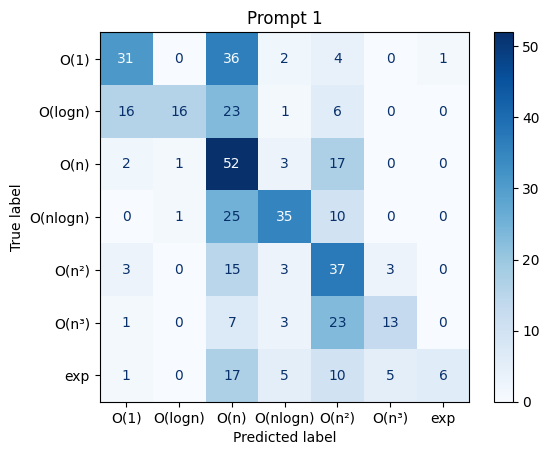
\includegraphics[width=0.7\textwidth]{CM_zeroshot_v1.png}
  \caption{Matriz de confusión haciendo zero-shot con el prompt 1}
  \label{fig:confmat_zs1}
\end{figure}

\begin{figure}[H]
  \centering
    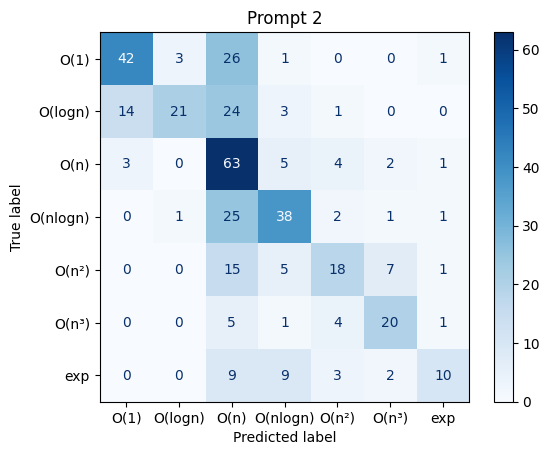
\includegraphics[width=0.7\textwidth]{CM_zeroshot_v2.png}
  \caption{Matriz de confusión haciendo zero-shot con el prompt 2}
  \label{fig:confmat_zs2}
\end{figure}

\begin{figure}[H]
  \centering
    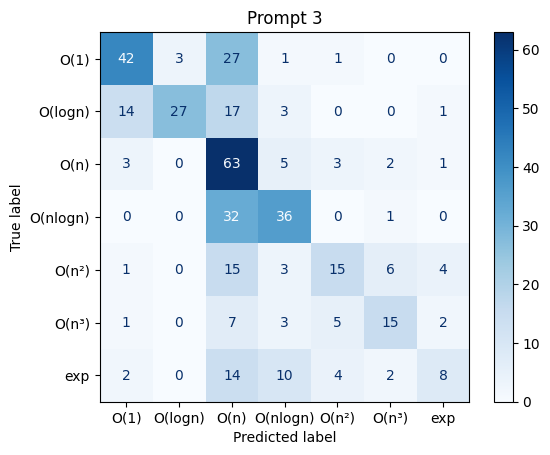
\includegraphics[width=0.7\textwidth]{CM_zeroshot_v3.png}
  \caption{Matriz de confusión haciendo zero-shot con el prompt 3}
  \label{fig:confmat_zs3}
\end{figure}

En la Tabla \ref{tab:tab_zs} podemos ver que la formulación del \textit{prompt} es un factor importante que repercute en los resultados del experimento, aunque en este caso las diferencias no son tan grandes. Con el \textit{prompt} 1 tenemos una exactitud de 41.8\%, pero al incluir las posibles clases de complejidad en el \textit{prompt} 2 conseguimos aumentarla hasta un 45\%. En el \textit{prompt} 3 se añaden aún más detalles, como especificar el rol del asistente como analista de complejidad computacional y delimitar el código con '///', pero esto solo acaba repercutiendo negativamente con una exactitud de 43.6\%. Así, el \textit{prompt} que mejores resultados ha obtenido es el \textit{prompt} 2.

En los tres \textit{prompts} tenemos que la clase mejor predicha es $\mathcal{O}(n)$ con exactitudes de 65\%, 75\% y 75\% respectivamente, mientras que la peor predicha es la exponencial con exactitudes de 12.8\%, 20\% y  16.7\% respectivamente, lo que sugiere una clara descompensación al predecir las distintas clases de complejidad.

En las Figuras \ref{fig:confmat_zs1}, \ref{fig:confmat_zs2} y \ref{fig:confmat_zs3} se aprecia que la clase predicha con mayor frecuencia es $\mathcal{O}(n)$, sin importar que haya sido correcta o no. Esto sugiere que el modelo tiene una mayor inclinación a asegurar que un código es de dicha clase de complejidad. Con el \textit{prompt} 2, el modelo suele confundir $\mathcal{O}(\log n)$ con $\mathcal{O}(1)$, exponencial con $\mathcal{O}(n\log n)$ y la mayoría de clases con $\mathcal{O}(n)$.

A continuación se muestran algunos ejemplos de códigos catalogados con el \textit{prompt} 2:

\begin{tcolorbox}[
  colback=gray!5,
  colframe=black,
  boxrule=0.5pt,
  breakable,
  title=$\mathcal{O}(\log n)$ catalogado como $\mathcal{O}(1)$,
]
\begin{verbatim}
# -*- coding: utf-8 -*-
"""
Created on Mon Sep  7 22:59:16 2020 

@author: Dark Soul
"""
import math
[l,r]=list(map(int,input().split()))l=l^r
if l:
    l=int(math.log(l,2))
    l=(1<<(l+1))-1
    print(l)
else:
    print(0)
\end{verbatim}
\end{tcolorbox}

\begin{tcolorbox}[
  colback=gray!5,
  colframe=black,
  boxrule=0.5pt,
  breakable,
  title=$\mathcal{O}(\log n)$ catalogado correctamente,
]
\begin{verbatim}
n, s = list(map(int, input().split()))

def sum_of_digits(n):
        ans = 0
        for c in str(n):
                ans += int(c)
        return ans

while m - sum_of_digits(m) < s:
        m += 10
if m <= n:
        print(n - m + 1)
else:
        print(0)
\end{verbatim}
\end{tcolorbox}

\begin{tcolorbox}[
  colback=gray!5,
  colframe=black,
  boxrule=0.5pt,
  breakable,
  title=Exponencial catalogado como $\mathcal{O}(n\log n)$,
]
\begin{verbatim}
from collections import defaultdict
from math import gcd
from heapq import heappop, heappush
n = int(input())
A = list(map(int, input().split()))
B = list(map(int, input().split()))
hp = [(0, 0)]
dis = {0: 0}
seen = set()
while hp:
    _, x = heappop(hp)
    if x == 1:
        print(dis[x])
        break
    seen.add(x)
    for a, b in zip(A, B):
        y = gcd(x, a)
        if y not in dis or dis[y] > dis[x] + b:
            dis[y] = dis[x] + b
            heappush(hp, (dis[y], y))
else:
    print(-1)
\end{verbatim}
\end{tcolorbox}

\begin{tcolorbox}[
  colback=gray!5,
  colframe=black,
  boxrule=0.5pt,
  breakable,
  title=Exponencial catalogado correctamente,
]
\begin{verbatim}
n,l,r,x=map(int,input().split())
import math
z=list(map(int,input().split()))
count=0
for i in range(pow(2,len(z))):
    mini=math.inf
    maxa=0
    j=i
    inde=0
    sume=0
    while(j>0):
        if(j&1):
            sume+=z[inde]
            maxa=max(maxa,z[inde])
            mini=min(mini,z[inde])
        j=j>>1
        inde+=1
    if(maxa-mini>=x and l<=sume<=r):
        count+=1
print(count)
\end{verbatim}
\end{tcolorbox}

\subsection{Few-shot}

Se tomará el \textit{prompt} 2 para incluir los ejemplos, pues es el que mejores resultados ofrece según la Tabla \ref{tab:tab_zs}. Dichos ejemplos se tomarán aleatoriamente dentro del conjunto \textit{train}. Indicaremos por [CÓDIGO] el lugar donde se incluye el código a analizar por el modelo y por [EJEMPLO] el lugar donde se incluyen los distintos códigos de ejemplo.

\begin{tcolorbox}[
  colback=gray!5,
  colframe=black,
  boxrule=0.5pt,
  breakable,
  title=Prompt few-shot,
]
Analyze the time complexity of the following code.

Choose exactly one of the following options: O(1), O(logn), O(n), O(nlogn), O(n\textasciicircum2), O(n\textasciicircum3) or exponential (O(2\textasciicircum n), O(3\textasciicircum n), etc.).

Here are some examples:
\\[\baselineskip]
Example 1:

Code:

[EJEMPLO]

Complexity: O(1)
\\[\baselineskip]
Example 2:

Code:

[EJEMPLO]

Complexity: O(logn)
\\[\baselineskip]
Example 3:

Code:

[EJEMPLO]

Complexity: O(n)
\\[\baselineskip]
Example 4:

Code:

[EJEMPLO]

Complexity: O(nlogn)
\\[\baselineskip]
Example 5:

Code:

[EJEMPLO]

Complexity: O(n\textasciicircum2)
\\[\baselineskip]
Example 6:

Code:

[EJEMPLO]

Complexity: O(n\textasciicircum3)
\\[\baselineskip]
Example 7:

Code:

[EJEMPLO]

Complexity: exponential
\\[\baselineskip]
Now analyze this code:

Code:

[CÓDIGO]

Complexity:
\end{tcolorbox}

La Tabla \ref{tab:tab_fs} muestra los resultados obtenidos en términos de exactitud y F1, y la Figura \ref{fig:confmat_fs} muestra la matriz de confusión obtenida con \textit{few-shot}.

\begin{table}[H]
    \centering
    \small
    \begin{tabular}{c c c c c c c|c c}
        $\mathcal{O}(1)$ & $\mathcal{O}(\log n)$ & $\mathcal{O}(n)$ & $\mathcal{O}(n\log n)$ & $\mathcal{O}(n^2)$ & $\mathcal{O}(n^3)$ & exponencial & Exactitud & Macro F1 \\ \hline
        55.3 & 50.0 & 71.4 & 62.8 & 27.7 & 33.3 & 30.6 & 49.7 & 51.8
    \end{tabular}
    \normalsize
    \caption{Exactitud de la predicción de las clases de complejidad con few-shot}
    \label{tab:tab_fs}
\end{table}

\begin{figure}[H]
  \centering
    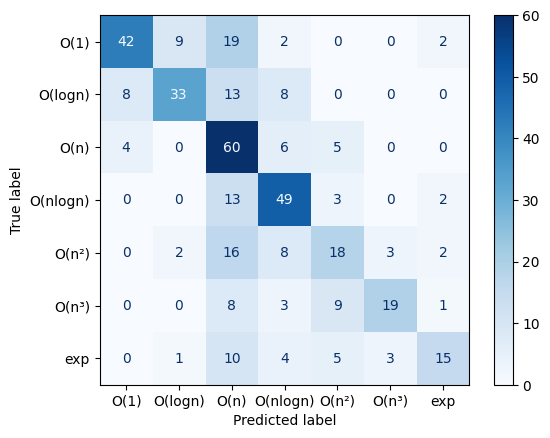
\includegraphics[width=0.7\textwidth]{CM_fewshot_v1.png}
  \caption{Matriz de confusión haciendo few-shot}
  \label{fig:confmat_fs}
\end{figure}

Según la Tabla \ref{tab:tab_fs}, los resultados mejoran al incorporar ejemplos al \textit{prompt}, lo que refuerza la idea del aprendizaje en contexto. Se obtiene una exactitud de 49.7\%, en comparación con el máximo 45\% que se obtuvo con \textit{zero-shot}. Además, exponencial ya no es la clase peor clasificada, sino $\mathcal{O}(n^2)$, con un 27.7\%, mientras que $\mathcal{O}(n)$ sigue siendo la mejor clasificada con un 71.4\%. Si lo comparamos con la Tabla \ref{tab:tab_zs}, la predicción de algunas clases ha mejorado, mientras que la de otras ha empeorado ligeramente. El resultado son unas predicciones algo más equilibradas que con \textit{zero-shot}.

Viendo la Figura \ref{fig:confmat_fs} podemos apreciar que sigue habiendo una predominancia por asignar la clase de complejidad $\mathcal{O}(n)$, pero ha mejorado ligeramente. Las confusiones más comunes en la matriz de confusión son: $\mathcal{O}(1)$ con $\mathcal{O}(\log n)$ y viceversa, $\mathcal{O}(\log n)$ con $\mathcal{O}(n\log n)$, $\mathcal{O}(n^2)$ con $\mathcal{O}(n\log n)$, $\mathcal{O}(n^3)$ con $\mathcal{O}(n^2)$ y todas las clases con $\mathcal{O}(n)$.

A continuación se muestran algunos ejemplos de códigos catalogados con \textit{few-shot}:

\begin{tcolorbox}[
  colback=gray!5,
  colframe=black,
  boxrule=0.5pt,
  breakable,
  title=$\mathcal{O}(1)$ catalogado como $\mathcal{O}(\log n)$,
]
\begin{verbatim}
def gcd(a,b):
    if b==0:
        return a
    else:
        return gcd(b,a%b)

if __name__ == "__main__":
    n = int(input())
    ans = 0
    if n==1:
        ans = 1
    elif n==2:
        ans = 2
    else:
        if n%2!=0:
            ans = n*(n-1)*(n-2)
        else:
            if gcd(n,(n-3)) ==1:
                ans = n*(n-1)*(n-3)
            else:
                ans = (n-1)*(n-2)*(n-3)
    print(ans)
\end{verbatim}
\end{tcolorbox}

\begin{tcolorbox}[
  colback=gray!5,
  colframe=black,
  boxrule=0.5pt,
  breakable,
  title=$\mathcal{O}(1)$ catalogado correctamente,
]
\begin{verbatim}
n=int(input())
if n==1 or n==2 :
    print(n)
elif n%2!=0 :
    m=n*(n-1)*(n-2)
    print(m)
elif n%3!=0 :
    m=n*(n-1)*(n-3)
    print(m)
else :
    m=(n-1)*(n-2)*(n-3)
    print(m)
\end{verbatim}
\end{tcolorbox}

\begin{tcolorbox}[
  colback=gray!5,
  colframe=black,
  boxrule=0.5pt,
  breakable,
  title=$\mathcal{O}(n^3)$ catalogado como $\mathcal{O}(n^2)$,
]
\begin{verbatim}
from sys import stdin
s=stdin.readline()
for ln in range(len(s),0,-1):
    for L in range(len(s)-ln+1):
        if s[L:L+ln] in s[L+1:]:
            print(ln)
            exit()
print(0)
\end{verbatim}
\end{tcolorbox}

\begin{tcolorbox}[
  colback=gray!5,
  colframe=black,
  boxrule=0.5pt,
  breakable,
  title=$\mathcal{O}(n^3)$ catalogado correctamente,
]
\begin{verbatim}
import sys
input = lambda: sys.stdin.readline().rstrip()

N, M, K = map(int, input().split())
if K % 2:
    for _ in range(N):
        print(*[-1] * M)
    exit()
A = [[int(a) for a in input().split()] for _ in range(N)]
B = [[int(a) for a in input().split()] for _ in range(N-1)]
X = [[0] * M for _ in range(N)]
inf = 1 << 30
for k in range(1, K // 2 + 1):
    nX = [[inf] * M for _ in range(N)]
    for i in range(N):
        for j in range(M):
            if i: nX[i][j] = min(nX[i][j], X[i-1][j] + B[i-1][j])
            if i < N - 1: nX[i][j] = min(nX[i][j], X[i+1][j] + B[i][j])
            if j: nX[i][j] = min(nX[i][j], X[i][j-1] + A[i][j-1])
            if j < M - 1: nX[i][j] = min(nX[i][j], X[i][j+1] + A[i][j])
    X = nX
for x in X:
    print(*[a * 2 for a in x])
\end{verbatim}
\end{tcolorbox}

\subsection{Modelo ajustado}

Para el modelo ajustado se ha escogido el \textit{prompt} 2 usado en \textit{zero-shot} pues presenta el mejor rendimiento según la Tabla \ref{tab:tab_zs} y ya no son necesarios los ejemplos de \textit{few-shot}. El modelo ha sido ajustado tres veces con distintos números de pasos: 60 pasos, 1 época (537 pasos) y 2 épocas (1074 pasos). Una época se corresponde con entrenar el modelo con el conjunto de entrenamiento completo; la cantidad de pasos depende del tamaño del conjunto de entrenamiento y de los parámetros escogidos al realizar el entrenamiento.

La Tabla \ref{tab:tab_QLoRA} muestra los resultados obtenidos en términos de exactitud y F1 y las Figuras \ref{fig:confmat_QLoRA1}, \ref{fig:confmat_QLoRA2} y \ref{fig:confmat_QLoRA3} muestran las matrices de confusión para cada cantidad de pasos durante el ajuste fino, respectivamente.

\begin{table}[H]
    \centering
    \resizebox{\linewidth}{!}{
    \begin{tabular}{c|c c c c c c c|c c}
        Entrenamiento & $\mathcal{O}(1)$ & $\mathcal{O}(\log n)$ & $\mathcal{O}(n)$ & $\mathcal{O}(n\log n)$ & $\mathcal{O}(n^2)$ & $\mathcal{O}(n^3)$ & exponencial & Exactitud & Macro F1 \\ \hline
        60 pasos & 71.4 & 69.7 & 70.2 & 55.1 & 47.7 & 80.7 & 71.4 & 66.2 & 66.5 \\
        1 época & 88.3 & 98.5 & 83.3 & 87.2 & 86.2 & 96.5 & 95.9 & 90.1 & 90.6 \\
        2 épocas & 85.7 & 93.9 & 91.7 & 88.5 & 89.2 & 100 & 91.8 & 91.2 & 91.8 
    \end{tabular}
    }
    \caption{Exactitud de la predicción de las clases de complejidad haciendo ajuste fino}
    \label{tab:tab_QLoRA}
\end{table}

\begin{figure}[H]
  \centering
    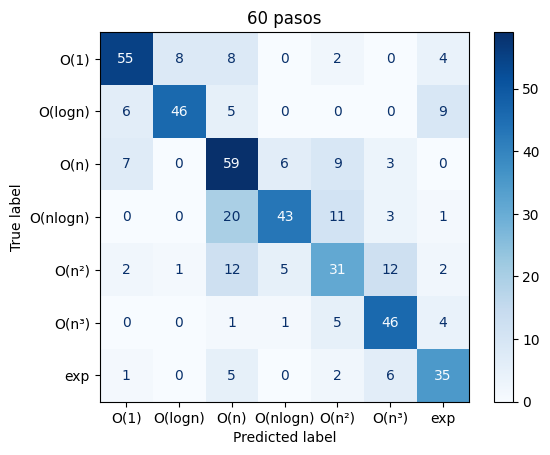
\includegraphics[width=0.7\textwidth]{CM_QLoRA_v1.png}
  \caption{Matrices de confusión haciendo ajuste fino con 60 pasos}
  \label{fig:confmat_QLoRA1}
\end{figure}

\begin{figure}[H]
  \centering
    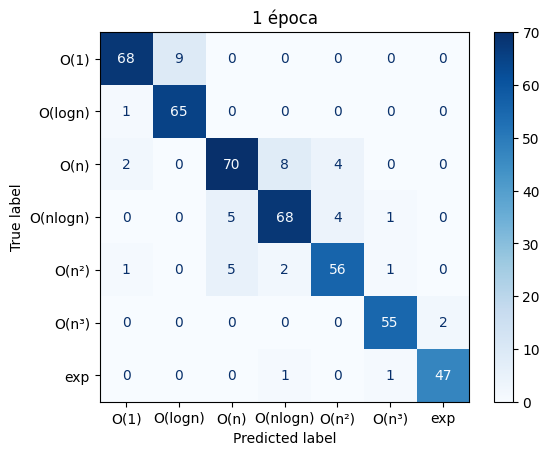
\includegraphics[width=0.7\textwidth]{CM_QLoRA_v2.png}
  \caption{Matrices de confusión haciendo ajuste fino con 1 época}
  \label{fig:confmat_QLoRA2}
\end{figure}

\begin{figure}[H]
  \centering
    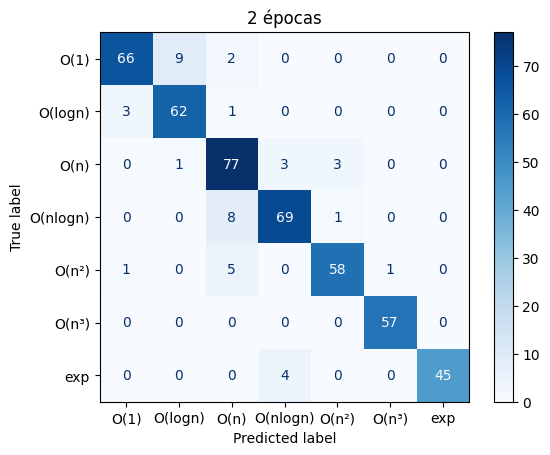
\includegraphics[width=0.7\textwidth]{CM_QLoRA_v3.png}
  \caption{Matrices de confusión haciendo ajuste fino con 2 épocas}
  \label{fig:confmat_QLoRA3}
\end{figure}

Comparando la Tabla \ref{tab:tab_QLoRA} con las Tablas \ref{tab:tab_zs} y \ref{tab:tab_zs} se ve claramente que el ajuste fino ha mejorado notablemente los resultados del experimento. Así podemos comprobar que la incorporación de numerosos ejemplos de una tarea a los datos de entrenamiento permite que el modelo pueda especializarse en dicha tarea, en este caso, analizar la complejidad computacional de un algoritmo. Además, aumentar la cantidad de pasos (y, en consecuencia, de ejemplos) durante el ajuste fino favorece el aprendizaje del modelo, incluso iterando varias veces sobre el mismo conjunto de datos, como es el caso del ajuste con 2 épocas.

En términos globales, el ajuste fino ha mejorado el modelo hasta alcanzar unas exactitudes de 66.2\%, 90.1\% y 91.2\%, habiendo sido entrenado con 60 pasos, 1 época y 2 épocas, respectivamente. Aunque es cierto que en términos globales el modelo ha mejorado su rendimiento con un mayor número de pasos, hay algunas clases que han empeorado sus predicciones de forma individual, pero esto se ve compensado con el resto de clases. La clase $\mathcal{O}(n^3)$ tiene una exactitud del 100\%, mientras que la clase peor predicha es $\mathcal{O}(1)$ con una exactitud de 85.7\%.

En las Figuras \ref{fig:confmat_QLoRA1}, \ref{fig:confmat_QLoRA2} y \ref{fig:confmat_QLoRA3} se aprecia la disminución de errores en las predicciones. Tras el ajuste fino de 2 épocas, los errores más comunes son confundir: $\mathcal{O}(1)$ con $\mathcal{O}(\log n)$, $\mathcal{O}(n\log n)$ con $\mathcal{O}(n)$, $\mathcal{O}(n^2)$ con $\mathcal{O}(n)$ y exponencial con $\mathcal{O}(n\log n)$.

A continuación se muestran algunos ejemplos de códigos catalogados con el ajuste fino de 2 épocas:

\begin{tcolorbox}[
  colback=gray!5,
  colframe=black,
  boxrule=0.5pt,
  breakable,
  title=$\mathcal{O}(n^2)$ catalogado como $\mathcal{O}(n)$,
]
\begin{verbatim}
n=int(input())
if n==1:
    print(1)
else:
    p=list(map(int,input().split()))
    children=[]
    for i in range(n):
        children.append([])
    for i in range(n-1):
        children[p[i]-1].append(i+1)
    layers=[1]+[0]*(n-1)
    layer=[0]
    num=2
    bylayer=[]
    while len(layer)>0:
        bylayer.append(layer)
        newlayer=[]
        for vert in layer:
            for child in children[vert]:
                layers[child]=num
                newlayer.append(child)
        layer=newlayer
        num+=1
    bylayer=bylayer[::-1]
    count=[0]*n
    for layer in bylayer:
        for vert in layer:
            if children[vert]==[]:
                count[vert]=1
            else:
                count[vert]=sum(count[v] for v in children[vert])
    count.sort()
    out=""
    for guy in count:
        out+=str(guy)+" "
    print(out)
\end{verbatim}
\end{tcolorbox}

\begin{tcolorbox}[
  colback=gray!5,
  colframe=black,
  boxrule=0.5pt,
  breakable,
  title=$\mathcal{O}(n^2)$ catalogado correctamente,
]
\begin{verbatim}
import sys
input=sys.stdin.buffer.readline
n,m=map(int,input().split())
for i in range(n//2+n%2):
    x1=i+1
    x2=n-i
    if(x1==x2):
        for j in range(m//2+m%2):
            if(j+1==m-j):
                sys.stdout.write((str(x1)+" "+str(j+1)+"\n"))
            else:
                sys.stdout.write((str(x1)+" "+str(j+1)+"\n"))
                sys.stdout.write((str(x2)+" "+str(m-j)+"\n"))
    else:
        if(i%2==0):
            for j in range(m):
                sys.stdout.write((str(x1)+" "+str(j+1)+"\n"))
                sys.stdout.write((str(x2)+" "+str(m-j)+"\n"))
        else:
            for j in range(m):
                sys.stdout.write((str(x1)+" "+str(m-j)+"\n"))
                sys.stdout.write((str(x2)+" "+str(j+1)+"\n"))
\end{verbatim}
\end{tcolorbox}

\begin{tcolorbox}[
  colback=gray!5,
  colframe=black,
  boxrule=0.5pt,
  breakable,
  title=$\mathcal{O}(n\log n)$ catalogado como $\mathcal{O}(n)$,
]
\begin{verbatim}
n = int(input())
p = list(map(int, input().split()))
gr = [[] for i in range(n)]
for i in range(n - 1):
    gr[p[i] - 1].append(i + 1)

q = [0]
after = []
i = 0
s = [0 for i in range(n)]
used = set()
used.add(0)
while q:
    cur = q.pop()
    after.append(cur)
    for el in gr[cur]:
        if el not in used:
            used.add(el)
            q.append(el)
            i += 1

q = after
for j in range(i, -1, -1):
    if len(gr[q[j]]) == 0:
        s[q[j]] = 1
    else:
        ans = 0
        for c in gr[q[j]]:
            ans += s[c]
        s[q[j]] = ans
s.sort()
print(' '.join(list(map(str, s))))
\end{verbatim}
\end{tcolorbox}

\begin{tcolorbox}[
  colback=gray!5,
  colframe=black,
  boxrule=0.5pt,
  breakable,
  title=$\mathcal{O}(n\log n)$ catalogado correctamente,
]
\begin{verbatim}
import sys
input_file = sys.stdin

[n,m] = list(int(x) for x in input_file.readline().split())
stacks = list(int(x) for x in input_file.readline().split())
stacks.sort()

ans = 0
cur_stack = 0
cur_h = 0

while cur_stack < n:
    ans += 1
    if stacks[cur_stack] >= cur_h + 1:
        cur_h += 1
    cur_stack += 1
ans += stacks[-1] - cur_h

print(sum(stacks) - ans)
\end{verbatim}
\end{tcolorbox}

\section{Conclusiones}

El objetivo principal de este trabajo era investigar si los grandes modelos de lengua (LLMs) pueden ser útiles para estimar automáticamente la complejidad computacional de algoritmos, sin necesidad de ejecutarlos ni realizar análisis manual. A partir de los resultados obtenidos en los experimentos, se puede concluir que este objetivo se ha cumplido satisfactoriamente, aunque no sin matices.

En primer lugar, se ha comprobado que los LLMs, incluso sin entrenamiento específico (\textit{zero-shot}), son capaces de realizar predicciones razonables sobre la complejidad de fragmentos de código, aunque su rendimiento es limitado. Este hecho evidencia que los LLMs han aprendido patrones generales sobre algoritmos y estructuras de control, pero no siempre son capaces de distinguir sutilezas entre clases de complejidad cercanas.

La inclusión de ejemplos (\textit{few-shot}) mejora el rendimiento, lo que refuerza la idea de que estos modelos son altamente sensibles al contexto proporcionado. No obstante, el mayor avance se ha conseguido mediante el ajuste fino. Tras entrenar el modelo con un conjunto de datos etiquetado, se ha alcanzado un 91\% de precisión y una F1 de 91,8\%, lo cual demuestra que los LLMs pueden adaptarse eficazmente a tareas de análisis algorítmico cuando se les proporciona la supervisión adecuada.

Desde un punto de vista crítico, este trabajo ha mostrado el potencial de los LLMs como herramientas de apoyo en la enseñanza, desarrollo y revisión de algoritmos, permitiendo obtener estimaciones rápidas de complejidad que pueden servir como punto de partida para un análisis más riguroso. No obstante, también se han identificado limitaciones importantes:

\begin{itemize}
    \item El modelo puede fallar cuando el código presenta ambigüedades, estructuras no convencionales o una lógica poco clara. Esto lo podemos ver en el siguiente ejemplo de código:

    \begin{tcolorbox}[
        colback=gray!5,
        colframe=black,
        boxrule=0.5pt,
        breakable,
        title=$\mathcal{O}(n)$ catalogado como $\mathcal{O}(n^2)$ con ajuste fino de 2 épocas,
    ]
    \begin{verbatim}
# your code goes here
import sys
n=int(input())
s=input()
s+=s
h=0
for i in range(n):
        if s[i]=='H':
                h+=1
ans=h
for i in range(n):
        c=0
        for j in range(i,i+h):
                if s[j]=='T':
                        c+=1
        ans=min(ans,c)
print(ans)
    \end{verbatim}
    \end{tcolorbox}

    donde la presencia de bucles anidados puede haber confundido al modelo.
    
    \item El modelo ajustado ha sido entrenado sobre un único lenguaje (\texttt{Python}) y un conjunto limitado de fragmentos, por lo que no se puede garantizar su generalización a otros lenguajes o problemas más complejos.
\end{itemize}

Cabe señalar que el alcance del trabajo se ha visto limitado por los recursos computacionales disponibles y por la necesidad de trabajar con modelos accesibles y conjuntos de datos ya existentes. Además, el conjunto de datos usado contiene considerables ejemplos de códigos extremadamente parecidos, incluso ya habiendo sido eliminados del conjunto de datos los que fueran idénticos entre sí, por lo que la fiabilidad de dicho conjunto entra en duda.

En resumen, este trabajo ha validado empíricamente la viabilidad de usar grandes modelos de lengua para estimar la complejidad computacional de algoritmos de forma automática. Aunque no se propone como sustituto del análisis formal, sí abre una vía prometedora para su automatización parcial, lo que podría tener implicaciones relevantes en el ámbito educativo y en herramientas de desarrollo asistido por inteligencia artificial. Futuros trabajos podrán ampliar esta línea de investigación, abordando nuevos lenguajes, tareas más complejas y mecanismos que aumenten la interpretabilidad de las decisiones del modelo.

\addcontentsline{toc}{section}{Referencias}
\begin{thebibliography}{100}




\bibitem{antecedentes} Albert, J. V., Rabasa, F. J. F., \& Quetglás, G. M. (1998). \textit{Introducció a l’anàlisi i disseny d’algorismes}. Universitat de València.

\bibitem{LayerNorm} Ba, J. L., Kiros, J. R., \& Hinton, G. E. (2016). \textit{Layer normalization}. arXiv. \url{https://arxiv.org/abs/1607.06450}

\bibitem{CodeComplex} Baik, S.-Y., Hahn, J., Kim, J., Jeon, M., Han, Y.-S., \& Ko, S.-K. (2024). CodeComplex: Dataset for worst‑case time complexity prediction. arXiv. \url{https://doi.org/10.48550/arXiv.2401.08719}

\bibitem{in-context learning} Brown, T. B., Mann, B., Ryder, N., Subbiah, M., Kaplan, J., Dhariwal, P., \ldots\ \& Amodei, D. (2020). Language models are few-shot learners. \textit{Advances in Neural Information Processing Systems}, \textit{33}, 1877--1901. \url{https://arxiv.org/abs/2005.14165}

\bibitem{bits} Goldberg, D. (1991). What every computer scientist should know about floating-point arithmetic. \textit{ACM Computing Surveys (CSUR)}, \textit{23}(1), 5--48. \url{https://doi.org/10.1145/103162.103163}

\bibitem{LSTM} Hochreiter, S., \& Schmidhuber, J. (1997). Long short-term memory. \textit{Neural Computation}, \textit{9}(8), 1735--1780. \url{https://doi.org/10.1162/neco.1997.9.8.1735}

\bibitem{fine-tuning} Howard, J., \& Ruder, S. (2018). Universal language model fine-tuning for text classification. In \textit{Proceedings of the 56th Annual Meeting of the Association for Computational Linguistics (ACL)} (pp. 328--339). \url{https://doi.org/10.18653/v1/P18-1031}

\bibitem{Adam} Kingma, D. P., \& Ba, J. (2014). \textit{Adam: A method for stochastic optimization}. arXiv. \url{https://arxiv.org/abs/1412.6980}

\bibitem{AdamW} Loshchilov, I., \& Hutter, F. (2019). \textit{Decoupled weight decay regularization}. arXiv. \url{https://arxiv.org/abs/1711.05101}

\bibitem{quantization} Jacob, B., Kligys, S., Chen, B., Zhu, M., Tang, M., Howard, A., Adam, H., \& Kalenichenko, D. (2018). Quantization and training of neural networks for efficient integer-arithmetic-only inference. In \textit{Proceedings of the IEEE Conference on Computer Vision and Pattern Recognition (CVPR)} (pp. 2704--2713). \url{https://arxiv.org/abs/1712.05877}

\bibitem{libro} Jurafsky, D., \& Martin, J. H. (2025). \textit{Speech and language processing: An introduction to natural language processing, computational linguistics, and speech recognition with language models} (3rd ed.). Manuscript in preparation. \url{https://web.stanford.edu/~jurafsky/slp3}

\bibitem{ROUGE} Lin, C.-Y. (2004). ROUGE: A package for automatic evaluation of summaries. In \textit{Proceedings of the Workshop on Text Summarization Branches Out (WAS 2004)} (pp. 74--81). \url{https://aclanthology.org/W04-1013/}

\bibitem{BLEU} Papineni, K., Roukos, S., Ward, T., \& Zhu, W.-J. (2002). BLEU: A method for automatic evaluation of machine translation. In \textit{Proceedings of the 40th Annual Meeting of the Association for Computational Linguistics (ACL)} (pp. 311--318). \url{https://doi.org/10.3115/1073083.1073135}

\bibitem{F1} Rajpurkar, P., Zhang, J., Lopyrev, K., \& Liang, P. (2016). SQuAD: 100,000+ questions for machine comprehension of text. In \textit{Proceedings of the 2016 Conference on Empirical Methods in Natural Language Processing (EMNLP)} (pp. 2383--2392). \url{https://aclanthology.org/D16-1264/}

\bibitem{retropropagación} Rumelhart, D. E., Hinton, G. E., \& Williams, R. J. (1986). Learning representations by back-propagating errors. \textit{Nature}, \textit{323}(6088), 533--536. \url{https://doi.org/10.1038/323533a0}

\bibitem{Llama} Touvron, H., Nathan, L., Li, C., Raffel, C., Sanchez-Gonzalez, A., Chen, Y., \ldots\ \& LLaMA Team. (2024). The LLaMA 3 herd of models. arXiv. \url{https://arxiv.org/abs/2407.21783}

\bibitem{transformer} Vaswani, A., Shazeer, N., Parmar, N., Uszkoreit, J., Jones, L., Gomez, A. N., Kaiser, Ł., \& Polosukhin, I. (2017). Attention is all you need. In \textit{Advances in Neural Information Processing Systems} (Vol. 30). \url{https://papers.nips.cc/paper_files/paper/2017/file/3f5ee243547dee91fbd053c1c4a845aa-Paper.pdf}





\end{thebibliography}


%-------------------------------------------------------------------------------------------------------
\newpage
\appendix

\section{Detalles del desarrollo del trabajo}

\begin{table}[H]
    \centering
    \begin{tabular}{l c}
        \hline
        Tarea & Tiempo (horas) \\
        \hline
        Recopilación de materiales & 20 \\
        Estudio de bibliografía & 20 \\
        Elaboración de resultados & 60 \\
        Redacción de la memoria & 50 \\
        \hline
        Total & 150 \\
        \hline
    \end{tabular}
    \caption{Tiempo aproximado de dedicación al trabajo}
    \label{tab:tiempo}
\end{table}

\begin{table}[H]
    \centering
    \begin{tabular}{l l p{7cm}}
        \hline
        Asignatura & Páginas & Descripción \\
        \hline
        Algoritmia & 5-7 & Definiciones y conceptos vistos en la asignatura \\
        Análisis de una variable real I & 6-7 & Se utilizan funciones de una variable real para representar los pasos de un algoritmo \\
        Análisis de varias variables reales I & 13 & Se calculan gradientes de funciones con varias variables reales \\
        Álgreba lineal I & 8-11, 14-15 & Conceptos básicos de álgebra lineal \\
        Probabilidad & 10-12, 14 & Se utilizan la renormalización y distribuciones de probabilidad \\
        Optimización II & 13 & Se usan métodos de optimización como descenso del gradiente \\ 
        Análisis de datos II & 16-30 & Se trabaja con métricas de rendimiento definidas en la asignatura \\
        \hline
    \end{tabular}
    \caption{Asignaturas relacionadas con el trabajo}
    \label{tab:asignaturas}
\end{table}

\end{document}